\chapter{Fundamentos}\label{ch:teory-reference}

\begin{flushright}
\textit{"Se eu vi mais longe, foi por estar sobre ombros de gigantes"}\\ (Isaac Newton)
\end{flushright}

% Resumo opcional. Comentar se não usar.
%\resumodocapitulo{}

%A primeira etapa de qualquer processo na engenharia é modelagem. A partir dela relacionamos todos conhecimentos relacionados a um sistema em busca de avaliar o comportamento através de uma descrição mais simplificada. Uma das principais formas é a modelagem matemática, em que é descrito as relações lógicas entre cada parte do sistema,. E assim, através de operações matemáticas podemos analisar em profundidade bem como extrapolar o estudo para sistema com modelos parecidos.

% Definição manipulador, resumo capítulo
Neste capítulo será apresentado os aspectos teóricos e técnicos das tecnologias envolvidas no controle implementado no manipulador robótico Meka A2. Segundo a ISO8373:2012, robôs são mecanismos de atuação programáveis em dois ou mais eixos com algum grau de autonomia, capazes de mover-se no ambiente em ordem de executar alguma tarefas. São dotados de sistemas de controle como forma de garantir a percepção e os acionamentos conforme solicitado \cite{nobody}. Manipuladores, por sua vez, são uma classe de robôs formados por uma série de segmentos conectados através de juntas ou com deslizamento entre si, com o propósito de pegar ou mover objetos de um lugar a outro \cite{nobody}. Para o desenvolvimento deste trabalho foi utilizado o manipulador robótico Meka A2. Sendo composto por 7 juntas com atuadores série elásticos. É um braço desenvolvido para pesquisa em tarefas em interação com pessoas de maneira segura em razão do baixo peso e da capacidade de ceder em contato com forças externas e por isto denominado complacente. O controle cinemático foi feito através de Quatérnions Duais, acrescentando mais uma camada ao controle em cascata das posições de junta já implementado.

\section{Manipuladores Robóticos} 

% Modelagem Matemática
Para controlar qualquer coisa é preciso definir um modelo matemático, que permita relacionar as características físicas às ações desejadas, permitindo assim que este seja comandado de alguma forma a partir das relações lógicas expressas no modelo usado. Em manipuladores robóticos o objeto de interesse para controle é o movimento no espaço como forma de permitir a execução da tarefa. Usualmente são adotadas duas abordagens denominadas cinemática e dinâmica.

% Modelagem Cinemática
Na cinemática estamos interessado apenas na geometria do movimento de pontos e objetos rígidos a partir da posição de cada ponto de referência e a variações no tempo, expressas como a velocidade e aceleração. Não são levados em conta as causas do movimento, isto é as forças e torques envolvidos.
% Introduzir representações cinemáticas, Matrizes Homogenias, ângulos de Euler, ...
% Servo Mecanismos - Controle de Posição apenas
% Segurança

% Na abordagem cinemática estamos interessado apenas no movimento em si independente das forças que o causaram. Desta forma são observados a posição, velocidade e aceleração de cada parte. Em um manipulador robótico, de forma geral, os movimentos são escolhidos com a finalidade da execução de uma tarefa envolvendo o uso de alguma ferramenta ou garra. Estas por sua vez são geralmente posicionadas no última junta por ser o ponto de maior alcance.

% Modelagem dinâmica, controle de torque
Na representação dinâmica, em oposição a cinemática, analisa as causa e efeitos do movimento através do estudo das forças envolvidas. Desta forma outras características são levadas em consideração como distribuição de massa de cada um dos segmentos e a interação com a força externas como a gravidade ou a interação com outros objetos. O que a torna uma representação mais complexa e computacionalmente mais cara. E também demanda do lado dos atuadores o controle de torque no lugar do controle de posição, sendo reservado inicialmente para aplicações em que o controle do torque no efetuador é crucial para a execução da tarefa.
% Alta impedância

% Este trabalho:

% Neste trabalho a posição e a orientação no espaço são representados a partir de Quatérnions Duais, o controle é feito por torque e não por posição e o braço é leve... esqueça tudo de clássico que a parada aqui é séria...

% Cada junta é controlada de maneira separada, assim para o controle da ponta é preciso converter o configuração das juntas somadas ao modelo geométrico das partes do braço para uma orientação e posição do efetuador no espaço em relação a base do manipulador.

\section{Quatérnions Duais}

% Representação da Posição e Orientação
Quatérnions Duais são números duais em que as partes primárias e secundárias são quatérnios \cite{nobody}.

\subsection{Quatérnions}
%
\subsection{Números Duais}
% Autodiferenciação

\subsection{Representação por Quatérnions Duais}

A representação em quatérnions duais traz como vantagens com relação a outras representações: eliminar as singularidades e a inexistência de ambiguidade de representação. Além de trazer uma representação mais compacta e portanto computacionalmente mais eficiente, uma vez que são utilizados 8 parâmetros ao invés de 12. % Citar paper IROS Bruno Adorno

São utilizados dois quatérnions, sendo um para a representação da posição e um quatérnion unitário para representação da orientação.

\subsection{DQ Robotics}

A representação do robô usando quatérnions duais é feita com auxílio da biblioteca DQ Robotics. Nela estão implementados as principais operações algébricas com Quarténions Duais bem como alguns controladores nas linguagens Matlab, Python e C++.

\section{Cinemática de Manipuladores}

\subsection{Descrição DH}

Cada barra do braço, pode ser descrita a partir dos dois pontos em cada uma das extremidades. Por sua vez cada um dos pontos é definido por 6 parâmetros, 3 para a posição em relação aos eixos x,y e z e 3 para orientação a partir da rotação em relação a cada um dos eixos. Somando 12 parâmetros para cada barra. Como forma de reduzir a quantidade de parâmetros necessários para cada link é adotado uma convenção baseada em apenas 4 valores denominada parâmetros de Denavit-Hatemberg. Cada barra é descrita a partir de 2 valores de distância e dois ângulos. Esta redução leva em conta que as partes do braço estão sempre conectadas e por tanto a descrição a partir dos pontos nas extremidade traria sempre redundância nos valores. Assim é descrito a relação entre cada um dos pontos através das medidas da distância e orientação dos encaixes nas extremidades de cada barra.

% Ilustração DH

% Configuração de junta?
Estes parâmetros são definidos de tal forma que apenas um possui variação com o acionamento. Em juntas prismáticas este representa variação da distância enquanto em enquanto em juntas cilíndricas um do ângulos que variam. O registro de posição atual de cada junta é referenciado como a configuração das juntas ou a pose do efetuador.

\subsection{Cinemática Direta}

A partir da descrição, é feito uma operação de mudança de transposição de plano para cada junta com o objetivo de relacionar a posição e orientação do efetuador em relação ao ponto da base. Para cada uma das juntas do braço é avaliado a variação da orientação e da posição em relação a extremidade da junta anterior. E assim, a partir da combinação destas operações em cadeia é possível determinar uma expressão relacionando a configuração de cada junta com a posição final.

\subsection{Cinemática Inversa}

A cinemática inversa consiste em identificar uma possível configuração de juntas que satisti

\subsection{Matrizes Homogenias}

% Jacobiano
\subsection{Cinemática Diferencial}

O problema da cinemática inversa nem sempre é simples de resolver e muitas vezes possui solução única. Uma forma de resolver é buscar uma solução aproximada na redondezas da posição atual.

Podemos entender o problema da cinemática inversa como um problema de mapeamento de uma região $R^n$ em uma representação de posição no espaço $(X,Y,Z)$ em conjunto de uma orientação $(Pich, Yaw, Row)$.

% Como forma de avaliar pequenas 

\section{Atuadores Série Elásticos}
% Controle de Torque e Complascência
% Modelo Proposto por Pratt

Cada uma juntas do Meka é um Atuador Série Elástico. Estes são uma implementação de atuador complacente descrito por Pratt e Williamson \cite{pratt1995series}. São basicamente constituídos de uma mola colocada em série entre um atuador e o ponto de saída e visam permitir uma maior segurança na operação com objetos rígidos, bem como na interação com outros robôs e pessoas. Em atuadores rígidos, o uso de redução permite que uma alta velocidade do motor seja traduzida em um alto torque gerando uma grande inércia. Assim, quando ocorre uma colisão, muita energia é transmitida ao objeto de contato bem como ao dente da engrenagem de saída, resultando internamente em um fratura no mecanismo da junta do robô. Ao se colocar um elemento elástico como uma mola, parte desta energia é absorvida e distribuída gradualmente reduzindo assim a possibilidade de fratura. De igual maneira a alta inércia representa um risco na execução de tarefas em conjunto com pessoa, pois um impacto nesta situação pode causar grande danos. Introduzir alguma forma de complacência é por norma \cite{nobody} um requisito de segurança para robô colaborativos ( co-bots ). Esta estrutura de atuador também facilita a interação entre manipuladores robóticos objetos rígidos, uma vez que a força percebida pelo atuador é reduzida pela contração interna da mola. O que por sua vez diminui a necessidade de alta precisão na operação como garantia de reduzir o esforço percebido pelo robô no contato com superfícies rígidas.

Tendo que a mola está em série entre o atuador e a carga, a contração da mola corresponde diretamente a força aplicada pelo motor na saída. O torque fornecido pode ser então obtido pela lei de Hooke ($T = k\cdot \Delta x$). Bastando que seja feita a medida da posição no atuador e na junta.

% Ilustração SEA

E desta forma a partir de medida de posição da motor e da junta após a mola o torque de saída pode ser medido e permite a implementação de um controle de torque preciso e de baixo custo como proposto \cite{nobody}. Em particular no Meka esta forma de atuação é implementado usando um motor Brushless em conjunto com um Harmonic drive e uma placa de controle DSP para controle do torque. O comportamento elástico é adicionado pela soma da elasticidade do Harmonic Drive e demais componentes na transmissão de cada junta e modulado pelo controlador de torque implementado por uma placa de controle embarcada dentro do braço. Desta forma a rigidez do atuador poder ser controlada via software como uma mola virtual. Em que a rigidez da mola é toda emulada por um sistema de controle a partir da referência do controle de posição e do controle de torque. Em resumo, quando a posição varia em relação a referência o controlador de baixo nível aumenta o torque de maneira proporcional ao erro da posição emulando o comportamento de uma mola, porém com rigidez totalmente ajustada pelo controlador. Desta forma a complacência e a rigidez pode ser ajustada dinamicamente por software. \cite{nobody}

Da mesma forma que o acréscimo de uma mola introduz uma maior segurança e permite um excelente controle de torque, traz o custo de uma menor precisão no controle de posição e algumas caraterísticas dinâmicas não desejadas como oscilações e respostas mais lentas.

%% Diagrama Atuadores Elásticos

% Uma das vantagens de atuadores série elásticos é permitir o controle de torque com precisão através de um controlador de posição. Isto é feito com base nas características dinâmicas da mola

%Do ponto de vista de controle, um atuador série elástico guarda semelhanças a um filtro passa-baixa, isto é, as variações bruscas como a colisão com algum obstáculo, são amortecidas enquanto variações baixas sofrem pouca alteração. No entanto tal acrescenta maior lentidão na resposta do sistema bem como introduz oscilações, uma vez que a energia acumulada pelos elementos elásticos será retransmitida gradualmente ao sistema.

% https://www.cc.gatech.edu/fac/Chris.Atkeson/legs/jh1c.pdf

\subsection{Encoder}

% Funcionamento Encoder
% Posição discreta e estimativa da Velocidade
% Torque obtido a partir da posição

Para cada junta são utilizados encoders para a medidas das grandezas a posição e o torque aplicado. Um enconder é tradicionalmente um sensor de posição. No entanto por conta da estrutura do atuador série elástico é possível avaliar também a torque aplicado na junta levando a em conta a dinâmica da mola, ou componente elástico do atuador. Desta forma o torque avaliado será a diferença da medida de posição da saída do motor e da junta vezes a rigidez da junta. 

\begin{figure}[H]
    \centering
    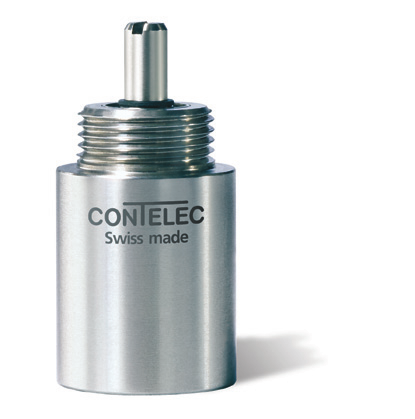
\includegraphics[width = 0.4\linewidth]{figs/vertX-encoder}
        \caption{Encoder utilizado nas juntas do robô}
    \label{fig:encoder}
\end{figure}

\subsection{Harmonic Drive}
% Descrição
% Modelo 

Harmonic Drive, também denominado "Engrenamento por ondas de deformação", é um sistema mecânico para redução de velocidade baseado no deslizamento de uma membrana flexível em torno de um engrenamento. É bastante popular na área de robótica por ter baixo deslizamento junto a uma alta capacidade de redução em um tamanho compacto. No entanto acrescenta atrito e flexibilidade às juntas. Esta característica de flexibilidade permite uma implementação extremamente compacta de um atuador série elástico, uma vez que rigidez possa ser modelada. Na figura \ref{fig:harmonic_drive}.

\begin{figure}[H]
    \centering
    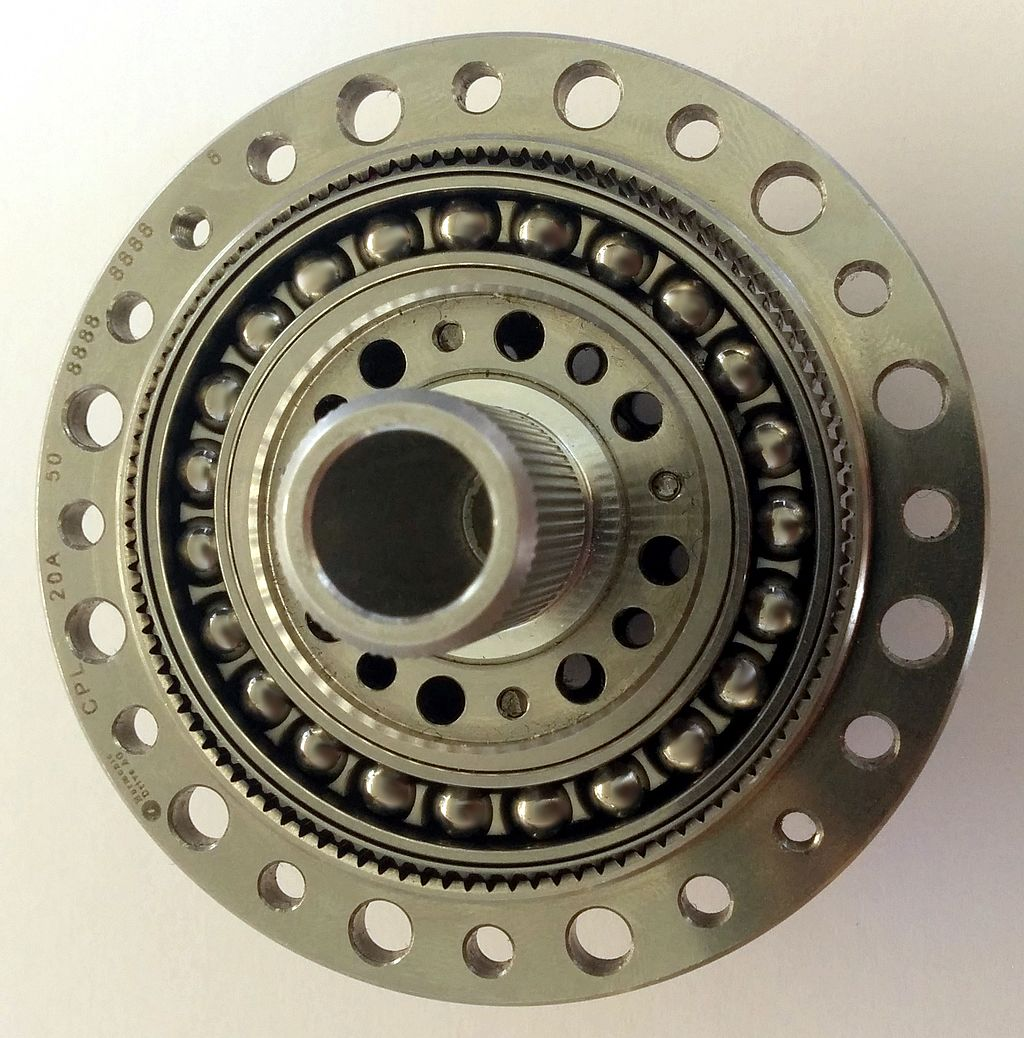
\includegraphics[width=0.4\linewidth]{tex/figs/harmonic_drive.jpg}
    \caption{Harmonic Drive (fonte: https://commons.wikimedia.org)}
    \label{fig:harmonic_drive}
\end{figure}

%% Porque é necessário colocar uma redução ?
%% Gráfico Torque vs Velocidade

% Características do Motor

% https://en.wikipedia.org/wiki/Harmonic_drive
% https://en.wikipedia.org/wiki/Strain_wave_gearing
% https://en.wikipedia.org/wiki/Backlash_(engineering)

\subsection{Motores Brushless}
% Descrição
% Comparativo com ServoMotores
Motores de corrente continua sem escovas ( comumente motores Brushless ) são motores síncronos controlados via corrente contínua. Oferecem baixa manutenção e alta performance pela redução do atrito entre as partes internas em relação a motores DC tradicionais. Tipicamente motores síncronos são controlados via corrente alternada e rotação é sincronizada com a frequência da tensão aplicada. Em um motor brushless é utilizado um inversor ou uma fonte chaveada para converter o sinal elétrico de corrente contínua em um sinal de corrente alternada com uma frequência definida. Desta forma, em conjunto com um circuito de controle interno em malha fechada, a velocidade pode ser ajustada e mantida com precisão. \cite{nobody} Nas figuras \ref{fig:maxon-servo} e \ref{fig:maxon-flat-servo} são mostrados dois dos motores utilizados no Meka.

\begin{figure}[H]
    \centering
    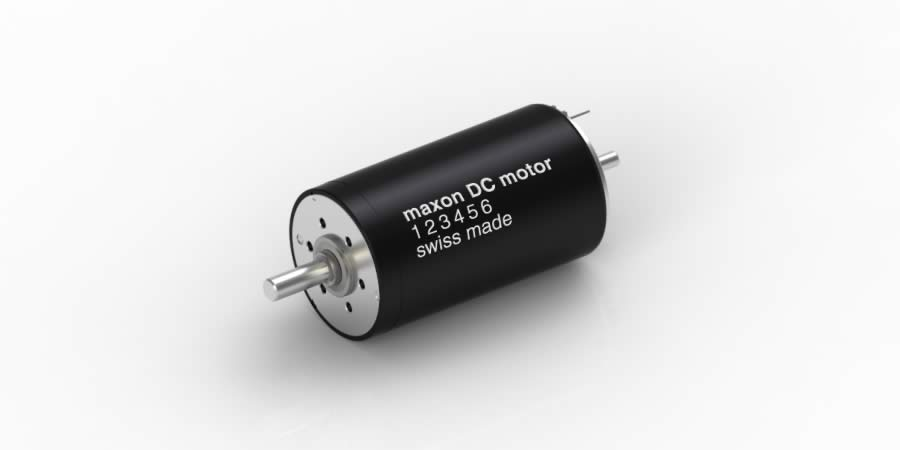
\includegraphics[width = 0.6\linewidth]{figs/maxon_servo.jpg}
    \caption{Motor utilizado nas juntas do Ombro}
    \label{fig:maxon-servo}
\end{figure}

\begin{figure}[H]
    \centering
    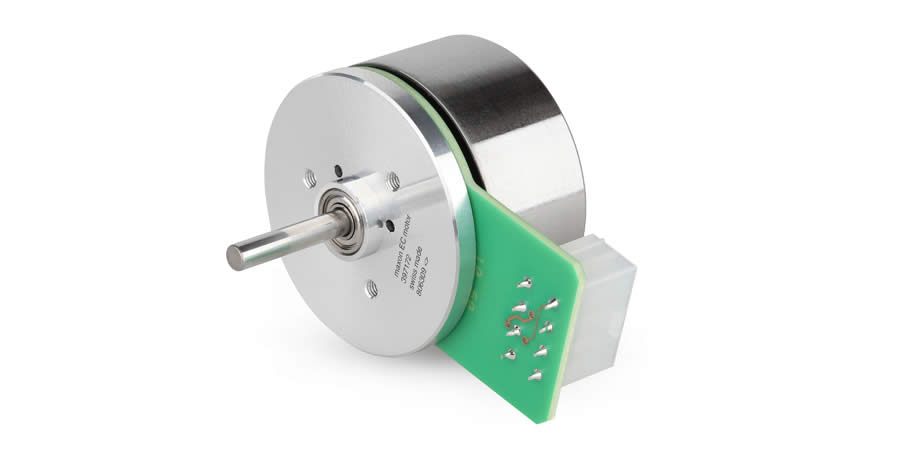
\includegraphics[width = 0.6\linewidth]{figs/maxon_flat_servo.jpg}
    \caption{Motor utilizado nas juntas do braço}
    \label{fig:maxon-flat-servo}
\end{figure}

% Comparativo com Motores DC
Em razão dos componentes eletrônicos usados para controle interno, motores Brushless são mais caros que motores magnéticos permanentes. No entanto, apresentam um custo de manutenção inferior uma vez que as partes internas estão sujeitas a um menor desgaste por atrito. Permitem um controle de velocidade preciso através do sensores de corrente por efeito Hall. Tendo ganhado espaço por garantirem um controle de velocidade melhor por um custo menor em comparação com servo-motores além de serem menores.

% Comparativo com Servo Motor
%% -> Servo Motor: controle de posição, torque e velocidade baseado em encoder
%% -> Motor Brushless: controle de velocidade baseado em sensor hall ( mais barato ), mais suave
% https://www.orientalmotor.com/brushless-dc-motors-gear-motors/technology/brushless-dc-motors-servo-motors-inverter.html

\section{Braço Robótico Meka A2}

% Descrição Meka
Cada uma das juntas do Meka A2 utiliza um atuador elástico composto por um motor Brushless em conjunto com uma redução baseada em engrenamento por onda de deformação, comercialmente denominado \textit{Harmonic Drive}. O controle é feito por placas DSP desenvolvidas pelo fabricante comandadas por sua vez por um computador embarcado conectado via Ethernet. Como forma de entender melhor o comportamento do robô, cada um destes componentes foi analisado de forma separada quanto as suas características de resposta no controle. 

\begin{figure}[H]
    \centering
    \includegraphics[width=0.6\linewidth]{figs/meka}
    \caption{Braço Robótico Meka A2}
    \label{fig:meka_arm}
\end{figure}

O controle é feito em cascata por uma série de controladores interagindo entre si. Cada nível opera na execução de uma tarefa possibilitando ao nível superior uma maior abstração do sistema e do objetivo a ser cumprido. Para garantir a estabilidade é preciso a dinâmica de cada controlador seja mais rápida. São estes, ordenados da dinâmica mais rápida para a mais lenta:

% Diagrama Controle em Cascata de Manipuladores
\begin{enumerate}
    \item Controladores do Motor ( velocidade e torque )
    \item Controle do Atuador Série Elástico ( posição, velocidade e torque )
    \item Controle de Posição do Efetuador ( Modelo Cinemático )
    \item Controlador de Trajetória
\end{enumerate}

%\subsection{Servo Controladores}
% Entrada como torque ou velocidade e saída posição

%Servo Controladores são controladores de posição a partir de uma referência  de torque ou velocidade. São geralmente associados a servo-motores, que são basicamente motores com esta estrutura de controle já implementada a partir de algum circuito eletrônico. No Meka, o controle de posição é feito pelo computador e não está incluído no atuadores. Este por sua vez traduz a referência do controle de posição em comandos serializados e enviados via EtherCAT para a placa de controle de torque.

%\subsection{Compensação da Gravidade}


% Matemática por trás
% Biblioteca Dinâmica
% Controle Feedforward

%\subsection{Controladores Cinemáticos}

\section{Sistema Embarcado}

O Meka é controlado pelo conjunto de dois sistema: um embarcado diretamente no braço para o controle da juntas e um externo sendo executado em PC com Ubuntu 12.04 com Kernel RTOS Xenomai em conjunto do sistema M3 da Meka Robotics e do framework ROS. No sistema embarcado são feita todas as interfaces com os sensores e atuadores. Enquanto no PC é feito o controle de cada uma das juntas e demais tarefas. A comunicação entre estes dois se dá por uma porta Ethernet e opera no protocolo proprietário EtherCAT. Desta forma é sistema pode ser facilmente expandido com o acréscimo de novos dispositivos e sensores.

\subsection{DSP Control Boards}
% Controle de torque
O controle de cada junta a partir do acionamento dos motores e da leitura dos sensores é feito pela placa DSP desenvolvida pela Meka Robotics. Nela estão implementados o controle de posição, velocidade, torque e rigidez de cada atuador. Cada uma das placas possui uma interface de comunicação EtherCAT ligada a um concentrador dentro do tronco do robô. Sendo este ligado através da porta Ethernet a um computador embarcado externo responsável pelo comando de cada uma das partes do robô.

\begin{figure}[H]
    \centering
    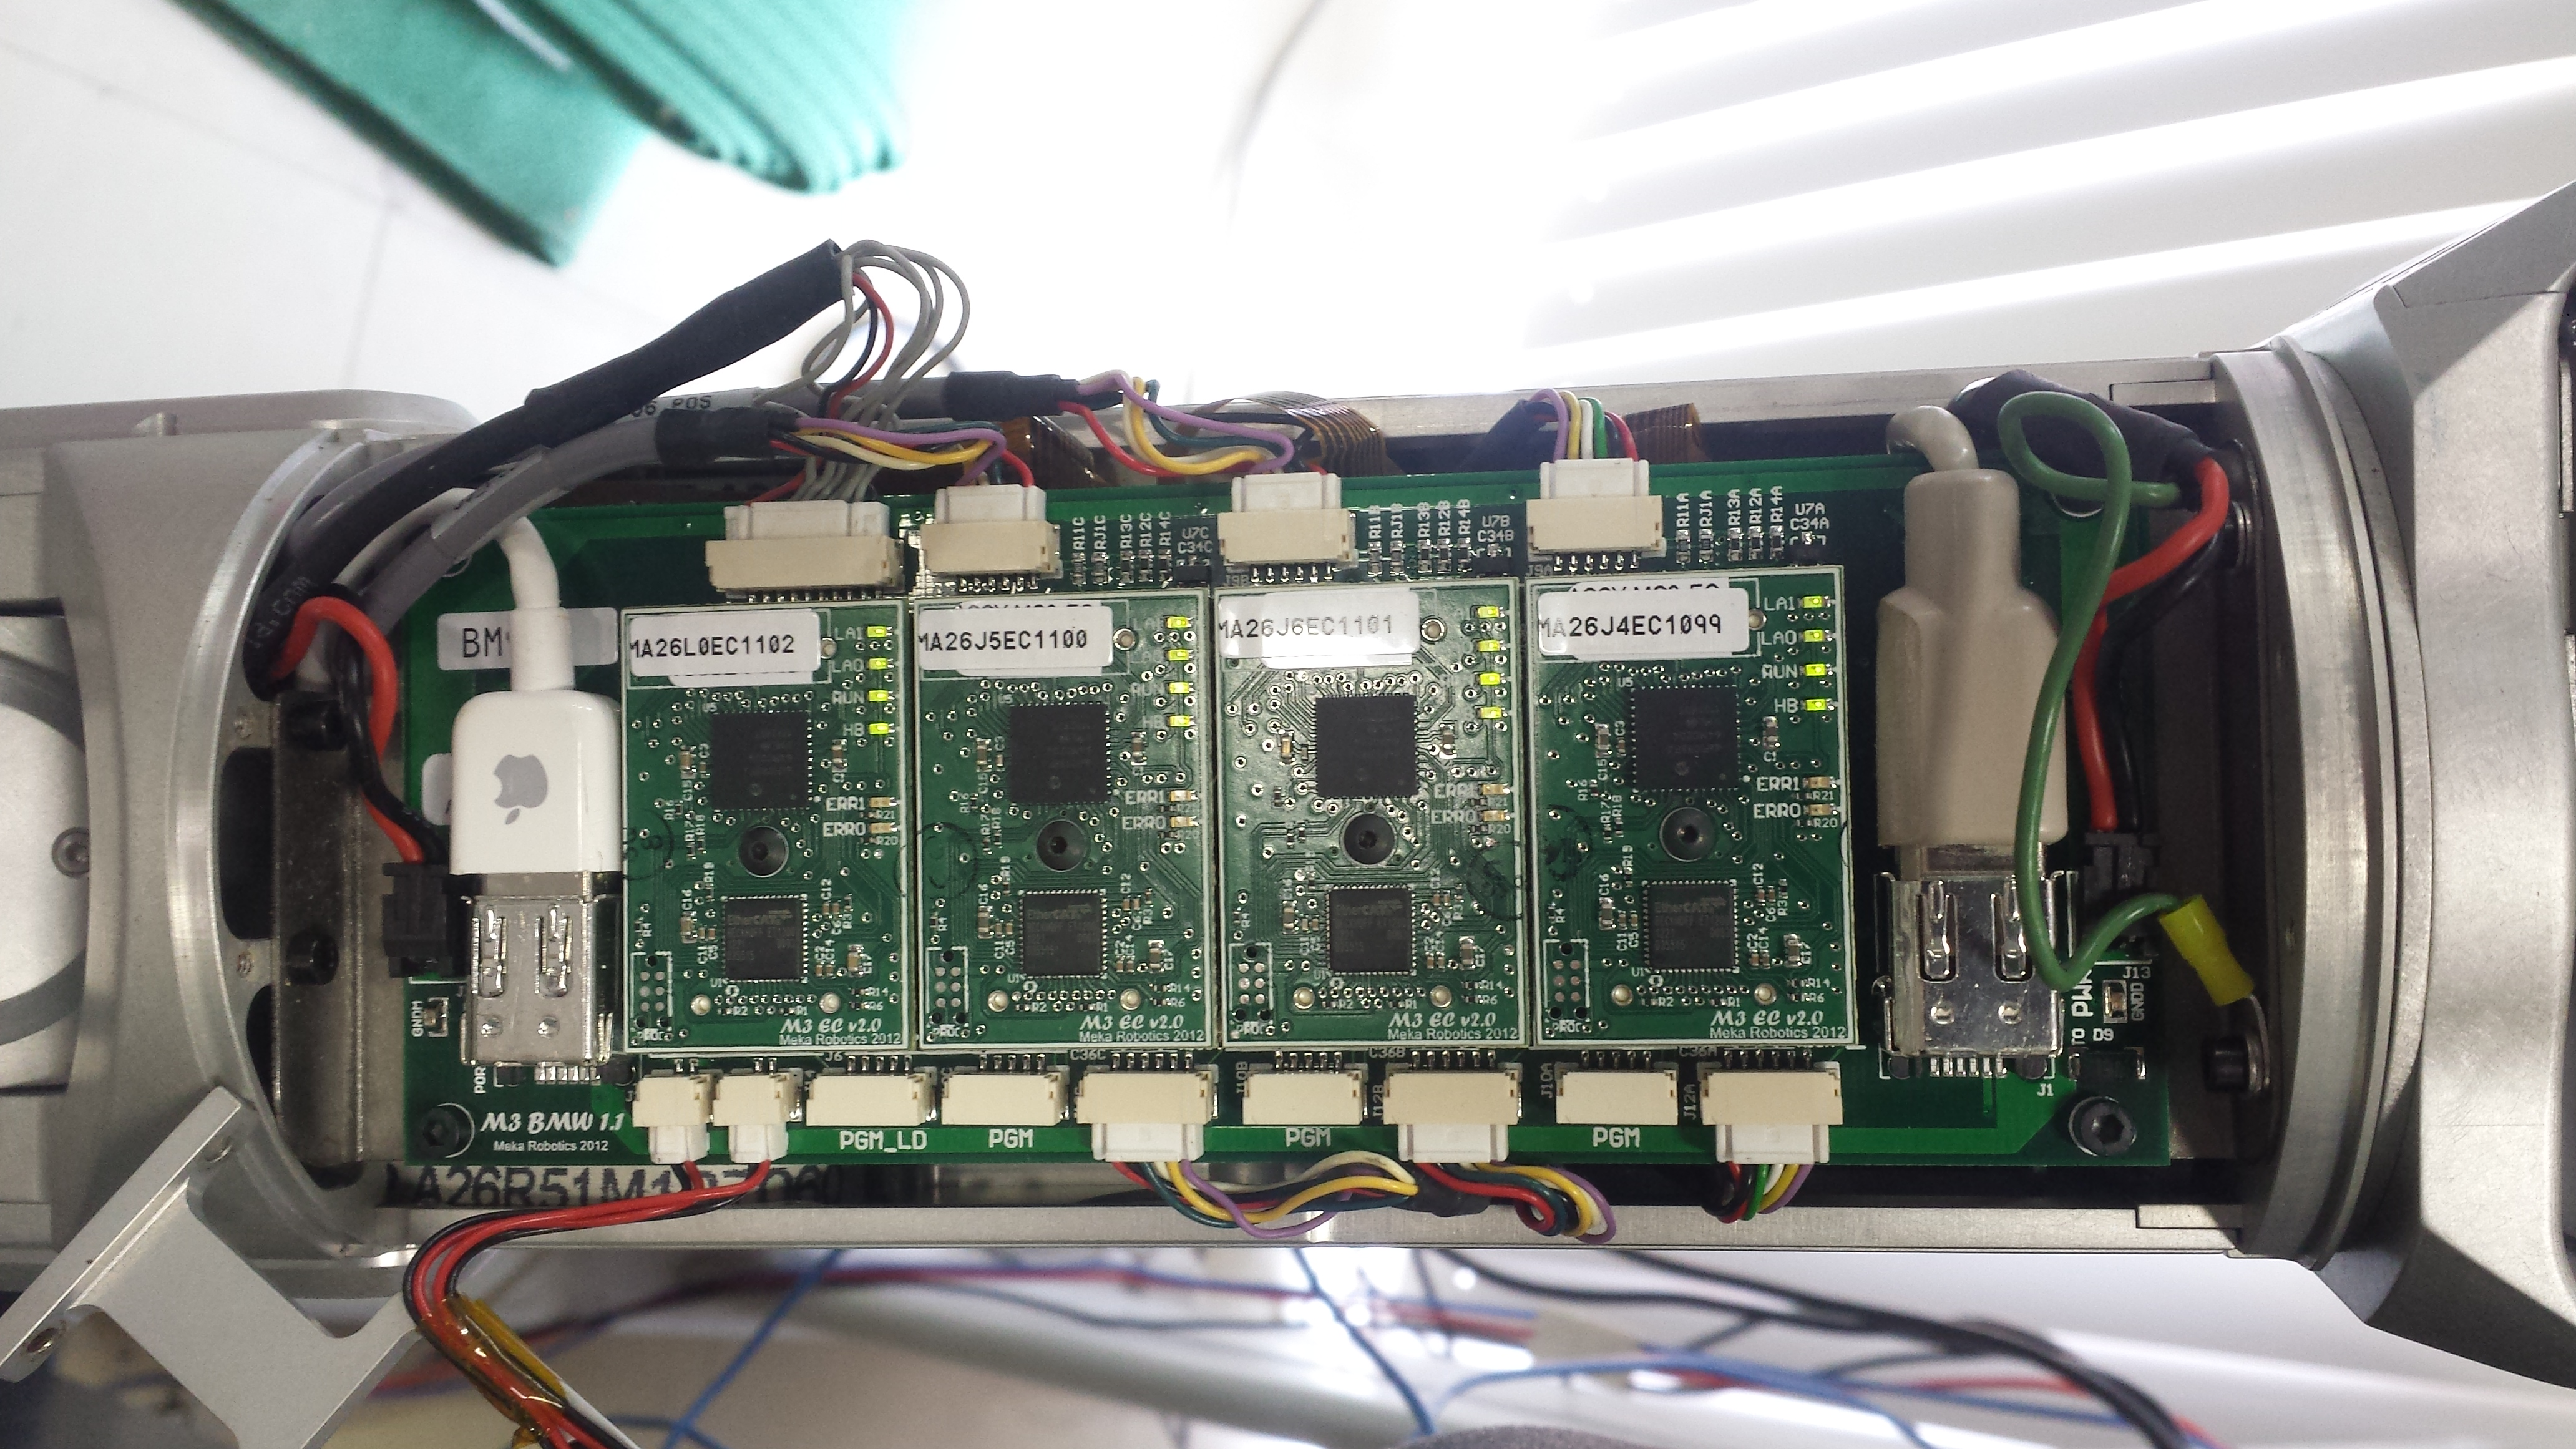
\includegraphics[width = 0.7\linewidth]{figs/dsp-control-wrist}
    \caption{Destaque Placas de controle dentro do braço \cite{nobody}}
    \label{fig:dsp-control-wrist}
\end{figure}

% Foto Portas Atrás 

\subsection{Meka PC}

Toda a parte de controle é feita no PC. Para iniciar a comunicação com o robô é executado um script que dispara os processos relacionados a comunicação com a robô via Socket pelo protocolo EtherCAT e a interface para Python. Um vez que o script está em execução o robô pode ser controlado por uma das interface da M3 entre elas a API em Python ou pelo ROS, conforme ilustrado no diagrama apresentado na figura \ref{fig:m3arch}.

% m3rt_server
% -> Interface via socket
% -> Memórica compartilhada
% -> API Python
% -> ROS
\section{M3}

M3 é o sistema de controle em tempo real para os robô desenvolvidos pela Meka Robotics. Representa core do robô em termos de controle e responde por todos acionamentos, sensores e ações do Meka. É bem extensa e baseada em módulos visando permitir a integração de múltiplos tipos de hardware. Possui código aberto e atualmente este encontra-se todo disponível nos repositórios do LARA \footnote{\url{https://github.com/lara-unb/Meka/tree/master/meka_robotics_source/mekabot}} e da Ensta Paris \footnote{\url{https://github.com/ahoarau/mekabot}}.

\begin{figure}[ht]
    \centering
    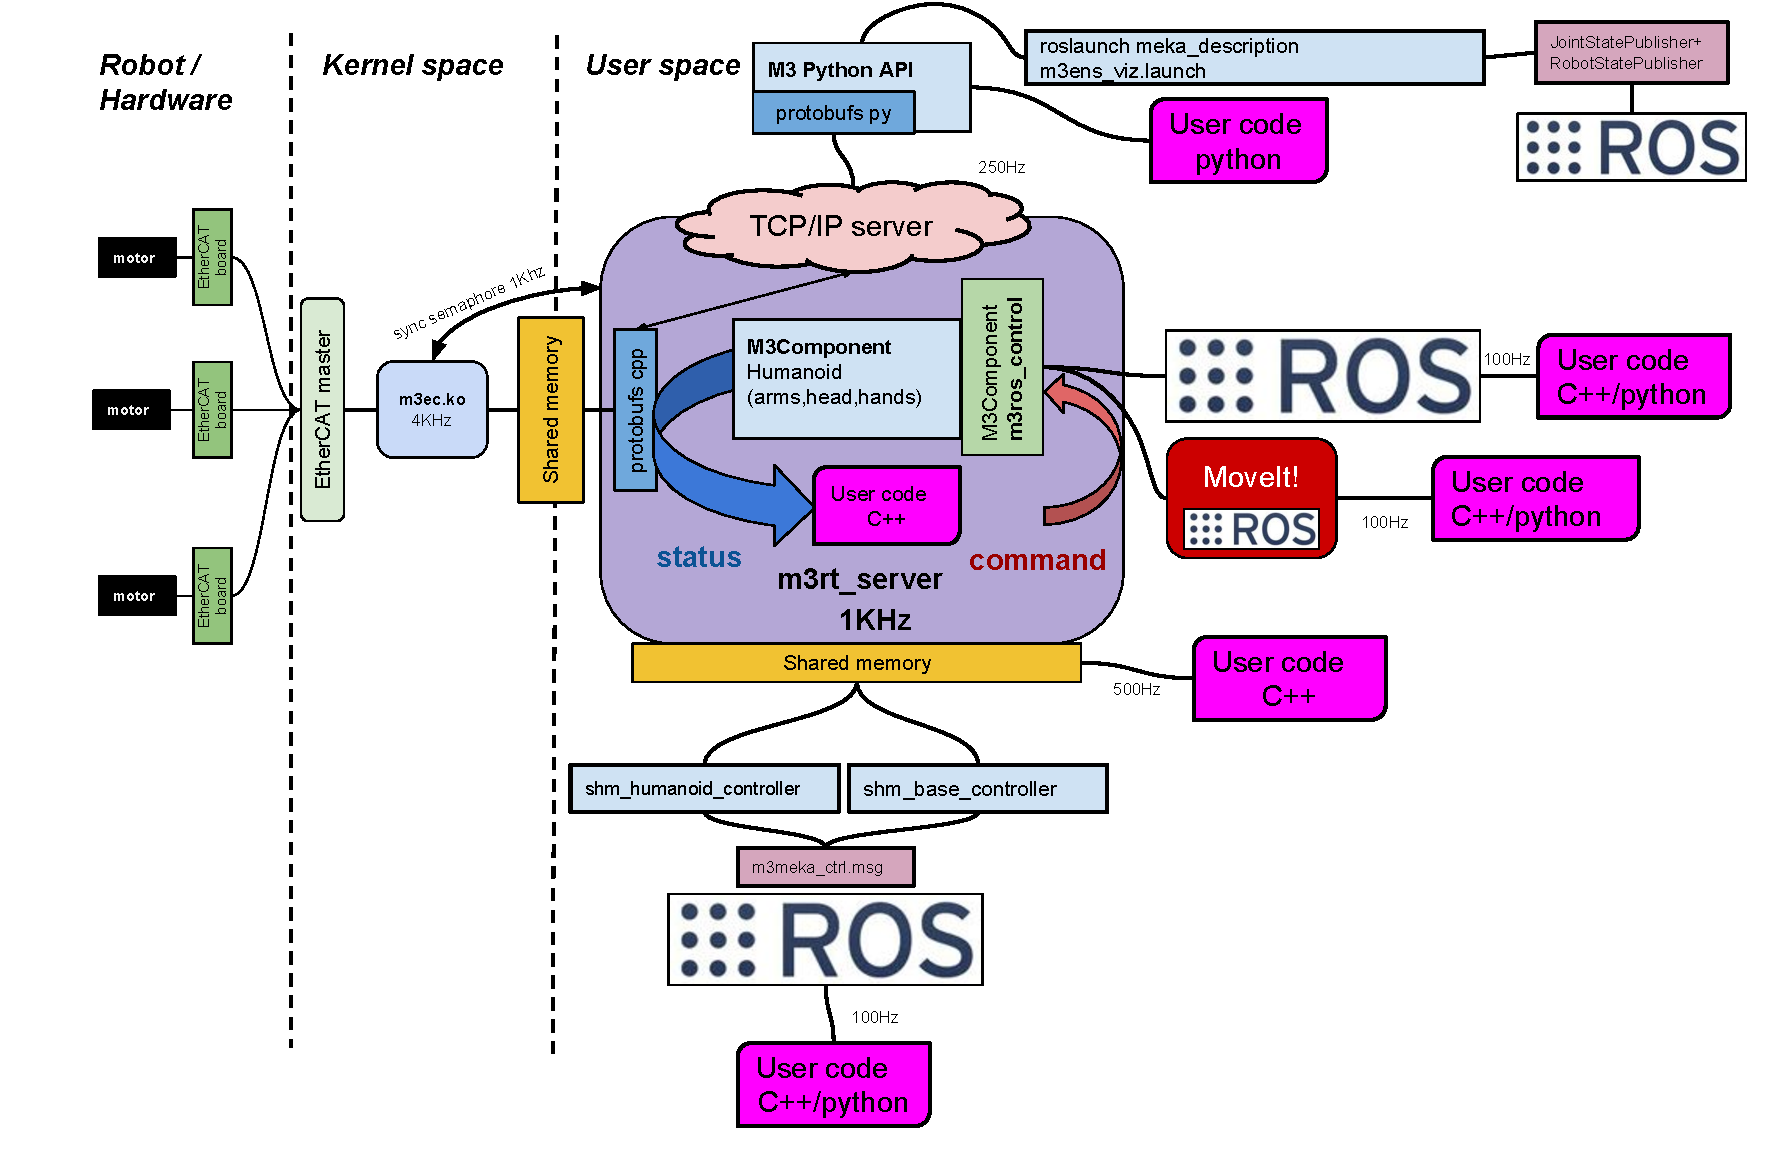
\includegraphics[width=\linewidth]{figs/m3_arch.pdf}
    \caption{Diagrama da arquitetura do robô \cite{hoarau_2015}}
    \label{fig:m3arch}
\end{figure}

% Descrição dos diretórios da m3

\subsection{Arquivos de Configuração}

Todas as configurações do Meka são guardadas através de arquivos $.yml$, localizados dentro da pasta $config$ de cada diretório. Em particular, dentro da pasta $m3ene$ estão tudo que é particular de configuração, drivers e ajuste para o funcionamento do robô do LARA. Esta pasta é baseada na $m3ens$ da Ensta Paris. Nela consta tudo para que o hardware completo disponível do robô e respectivos controladores funcionem, incluindo informações sobre sensor de força, atuadores, garra e parâmetros do modelo dinâmico do robô e da garra.

\subsection{ROS}

Robotics Operating System (ROS) é um \textit{framework} voltado para a robótica que reúne as melhores práticas para robótica em conjunto com um sistema de comunicação distribuída que permite o uso de diferentes linguagens de programação no mesmo projeto. Começou em 2007 reunindo conceitos de diversos projetos de software aberto anteriores e com o passar dos anos se tornou um padrão dentro da comunidade de robótica, contando com implementação para diversos robôs comerciais e inclusive uma versão completa voltada exclusivamente para a industria. \cite{nobody}



